\documentclass[a4paper]{report}
\usepackage[utf8]{inputenc}
\usepackage[portuguese]{babel}
\usepackage{hyperref}
\usepackage{a4wide}
\hypersetup{pdftitle={CG - Fase 1 - Grupo 7},
pdfauthor={João Teixeira, José Ferreira, Miguel Solino},
colorlinks=true,
urlcolor=blue,
linkcolor=black}
\usepackage{subcaption}
\usepackage[cache=false]{minted}
\usepackage{listings}
\usepackage{booktabs}
\usepackage{multirow}
\usepackage{appendix}
\usepackage{tikz}
\usepackage{authblk}
\usepackage{bashful}
\usepackage{verbatim}
\usepackage{amsmath}
\usepackage{tikz}
\usepackage{tikz,fullpage}
\usepackage{pgfgantt}
\usepackage{amssymb}
\usetikzlibrary{arrows,%
                petri,%
                topaths}%
\usepackage{tkz-berge}
\usetikzlibrary{positioning,automata,decorations.markings}
\AfterEndEnvironment{figure}{\noindent\ignorespaces}
\AfterEndEnvironment{table}{\noindent\ignorespaces}

\definecolor{solarized@base03}{HTML}{002B36}
\definecolor{solarized@base02}{HTML}{073642}
\definecolor{solarized@base01}{HTML}{586e75}
\definecolor{solarized@base00}{HTML}{657b83}
\definecolor{solarized@base0}{HTML}{839496}
\definecolor{solarized@base1}{HTML}{93a1a1}
\definecolor{solarized@base2}{HTML}{EEE8D5}
\definecolor{solarized@base3}{HTML}{FDF6E3}
\definecolor{solarized@yellow}{HTML}{B58900}
\definecolor{solarized@orange}{HTML}{CB4B16}
\definecolor{solarized@red}{HTML}{DC322F}
\definecolor{solarized@magenta}{HTML}{D33682}
\definecolor{solarized@violet}{HTML}{6C71C4}
\definecolor{solarized@blue}{HTML}{268BD2}
\definecolor{solarized@cyan}{HTML}{2AA198}
\definecolor{solarized@green}{HTML}{859900}

\lstset{
  language=Java,
  upquote=true,
  columns=fixed,
  tabsize=4,
  extendedchars=true,
  breaklines=true,
  numbers=left,
  numbersep=5pt,
  rulesepcolor=\color{solarized@base03},
  numberstyle=\tiny\color{solarized@base01},
  basicstyle=\footnotesize\ttfamily,
  keywordstyle=\color{solarized@green},
  stringstyle=\color{solarized@yellow}\ttfamily,
  identifierstyle=\color{solarized@blue},
  commentstyle=\color{solarized@base01},
  emphstyle=\color{solarized@red}
}

\begin{document}

\title{Computação Gráfica\\
\large Fase 1 - Grupo 7}
\author{José Ferreira (A83683) \and João Teixeira (A85504) \and Miguel Solino (A86435)}
\date{\today}

\begin{center}
    \begin{minipage}{0.75\linewidth}
        \centering
        
\includegraphics[width=0.4\textwidth]{images/eng.jpeg}\par\vspace{1cm}
        \vspace{1.5cm}
        \href{https://www.uminho.pt/PT}
        {\color{black}{\scshape\LARGE Universidade do Minho}} \par
        \vspace{1cm}
        \href{https://www.di.uminho.pt/}
        {\color{black}{\scshape\Large Departamento de Informática}} \par
        \vspace{1.5cm}
        \maketitle
    \end{minipage}
\end{center}

\tableofcontents

\chapter{Introdução}
Este trabalho foi desenvolvido no âmbito da unidade curricular de computação
gráfica e está dividido em várias fases de entrega distintas sendo que esta é a
primeira.\\
Esta fase está dividido em duas partes distintas, o \textit{generator} e o
\textit{engine}.\\
O \textit{generator} destina-se a gerar os pontos que desenham um conjunto de
primitivas.\\
O \textit{engine} destina-se a representar as primitivas produzidas
anteriormente.\\
De forma a facilitar a compilação do código foi criado um \textit{script}
chamado \textit{build.sh} que compila o código e gera os dois executáveis dentro
da pasta \textit{target/release/bin} quando executado.\\
Ao longo deste relatório irá ser explicado a metodologia e raciocínio usados
para a realização desta fase.\\

\chapter{Utils}
\section{Sistemas de Coordenadas}
De forma a facilitar o desenho das formas foram desenvolvidas um conjunto de
classes para representar dois sistemas distintos de coordenadas.\\
O primeiro sistema de coordenadas é o sistema cartesiano. Neste a posição de um
ponto no espaço fica definido com 3 valores: x, y e z.\\
\begin{figure}[H]
    \centering 
    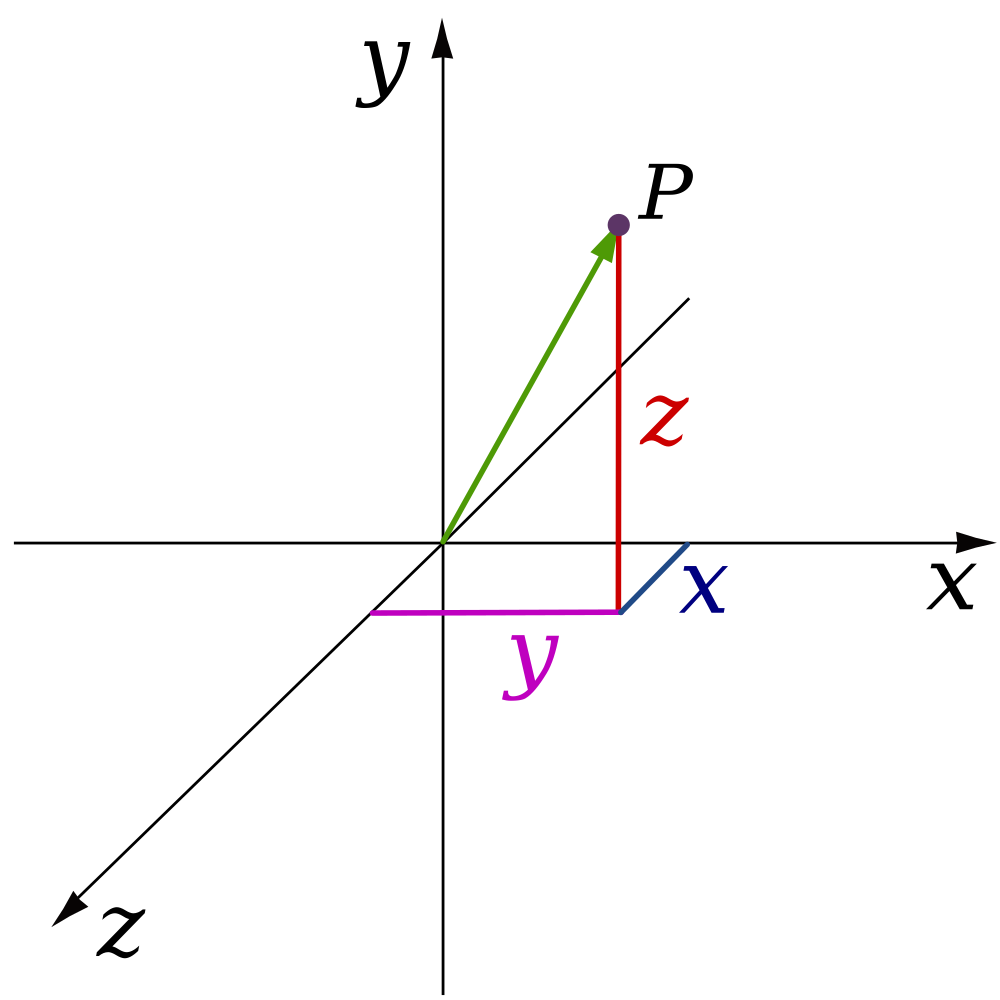
\includegraphics[width=0.25\textwidth]{images/Coord_XYZ.png}  
    \caption{Coordenadas cartesianas}
    \label{fig:coord_xyz}
\end{figure}
O segundo sistema de coordenadas é o sistema esférico. Neste, para definir a
posição de um ponto no espaço, são também necessários 3 valores: raio,
inclinação e azimute. O raio é a distancia que o ponto tem à origem do
referencial, a inclinação é o ângulo que o ponto faz com o eixo vertical e o
azimute é o ângulo que o ponto faz com o eixo dos z.
\begin{figure}[H]
    \centering 
    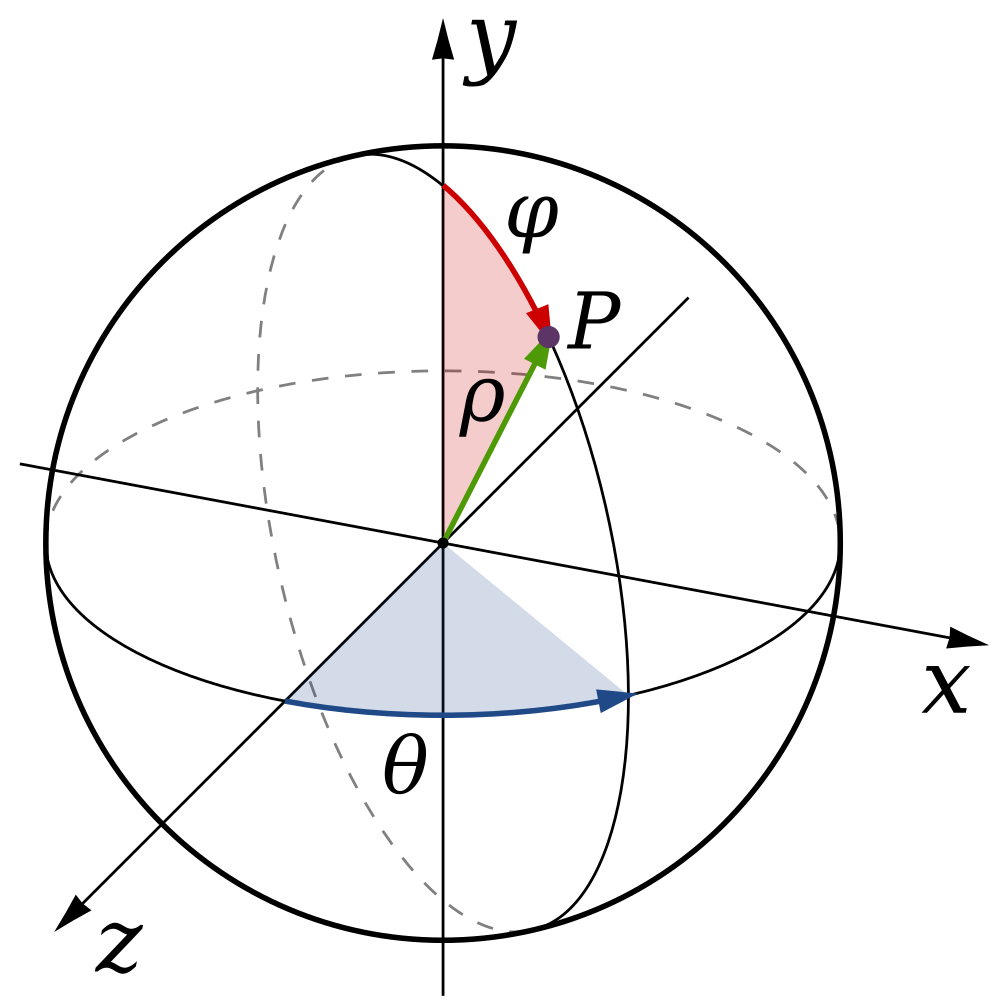
\includegraphics[width=0.25\textwidth]{images/Spherical_Coordinates.png}  
    \caption{Coordenadas esféricas}
    \label{fig:spherical_coordinates}
\end{figure}
Para ambos os sistemas de coordenadas foram definidos uma classe de pontos e uma
classe de vetores.\\
Também foram implementadas operações simples fazendo uso de \textit{operator
overloading} de forma a ser possível, por exemplo, escrever \textit{Point} +
\textit{Vector} e o resultado desta operação dar um \textit{Point}.

\chapter{Generator}
Neste módulo foram definidas 5 primitivas:
\begin{itemize}
        \item Plano
        \item Caixa
        \item Esfera
        \item Cone
        \item Cilindro
\end{itemize}
O formato escolhido para representar os pontos gerados é o de colocar um
ponto por linha com as coordenadas pela ordem X, Y e Z e separados por espaço.\\
Assim, por exemplo, o conjunto de pontos (0, 0, 0), (1, 0, 0) e (1, 1, 1)
ficaria representado como.
\begin{lstlisting}
0 0 0
1 0 0
1 1 1
\end{lstlisting}

\section{Plano}
Para desenhar um plano com dois triângulos sabendo o lado do plano basta
conseguir obter as coordenadas dos cantos do plano.\\
\begin{figure}[H]
    \centering 
    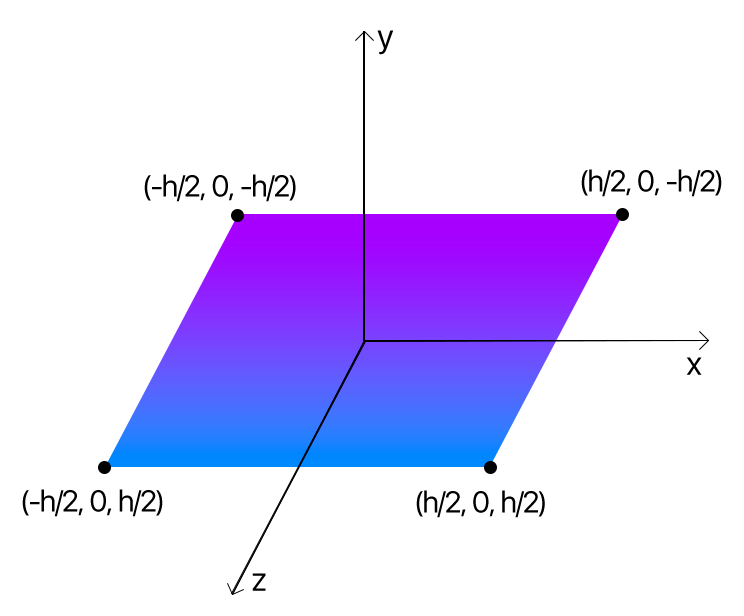
\includegraphics[width=0.5\textwidth]{images/esquema_plano.png}  
    \caption{Esquema dos pontos no plano}
    \label{fig:scheme_plane}
\end{figure}
Para desenhar um triângulo com o lado visível virado para cima é necessário
seguir a regra da mão direita quando se decide porque ordem desenhar os pontos.
Assim, os dois triângulos necessários são definidos da seguinte forma:\\
Para definir o triângulo superior:
\[(-h/2,\quad 0, \quad -h/2)\]
\[(-h/2,\quad  0, \quad h/2)\]
\[(h/2,\quad  0, \quad -h/2)\]
Para definir o triângulo inferior:
\[(h/2, \quad 0, \quad -h/2)\]
\[(-h/2, \quad  0, \quad  h/2)\]
\[(h/2, \quad  0, \quad h/2)\]

\begin{figure}[H]
    \centering 
    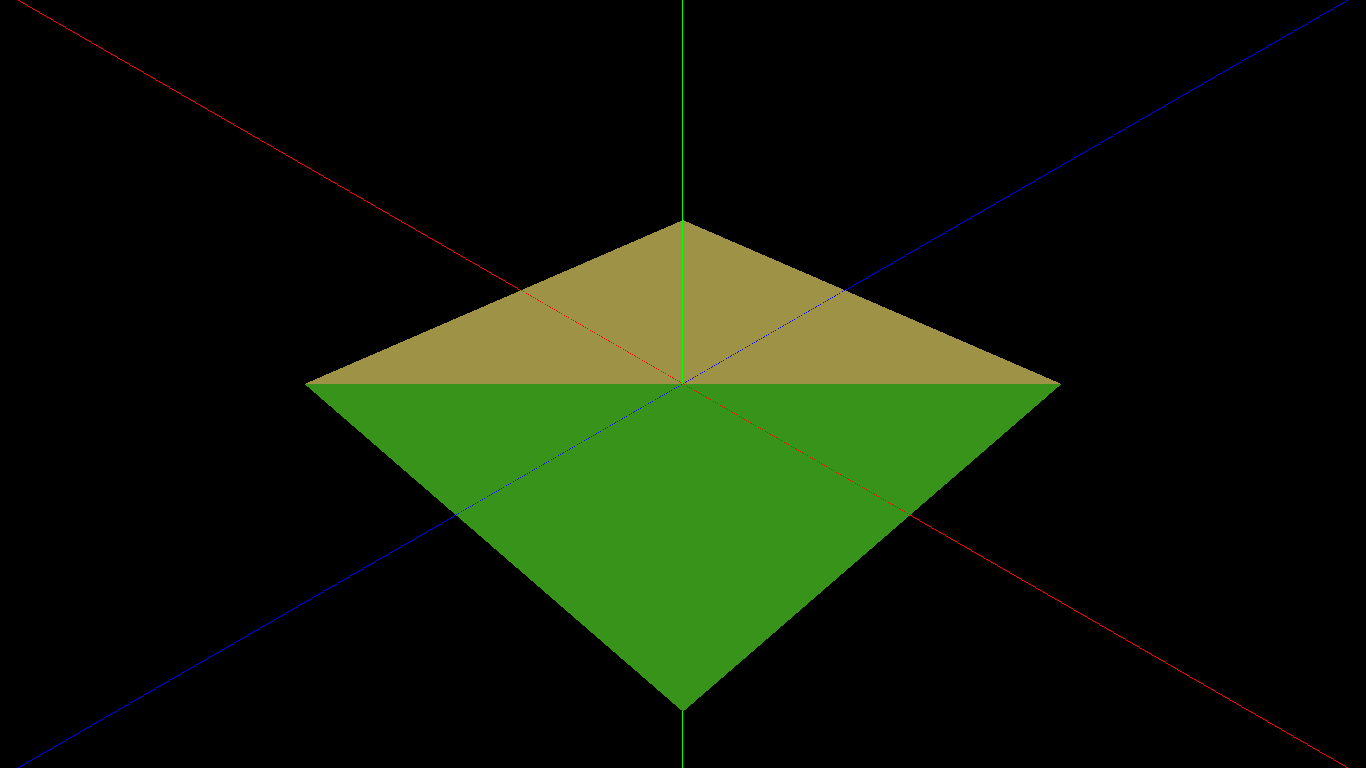
\includegraphics[width=0.5\textwidth]{images/plane.png}  
    \caption{Plano Side:10}
    \label{fig:plane}
\end{figure}

\section{Caixa}
Para desenhar uma caixa é necessário saber as dimensões da caixa (\textit{\_X},
\textit{\_Y}, \textit{\_Z}) e, opcionalmente, o número de divisões da caixa
(\textit{\_slices - 1}).\\
Para definir cada uma das faces de uma caixa é necessário ter um ponto que
esteja nessa face. De forma a minimizar os pontos que são definidos escolhemos
dois pontos em cantos opostos. Neste caso no canto inferior esquerdo da frente
(\textit{front}) e no canto superior direito de trás (\textit{back}):\\
\begin{lstlisting}
Point front  = Point(-_x/2, -_y/2,  _z/2);
Point back   = Point( _x/2,  _y/2, -_z/2);
\end{lstlisting}
Assim, todas as faces da caixa podem ser definidas com base em apenas dois
pontos.\\
\begin{figure}[H]
    \centering 
    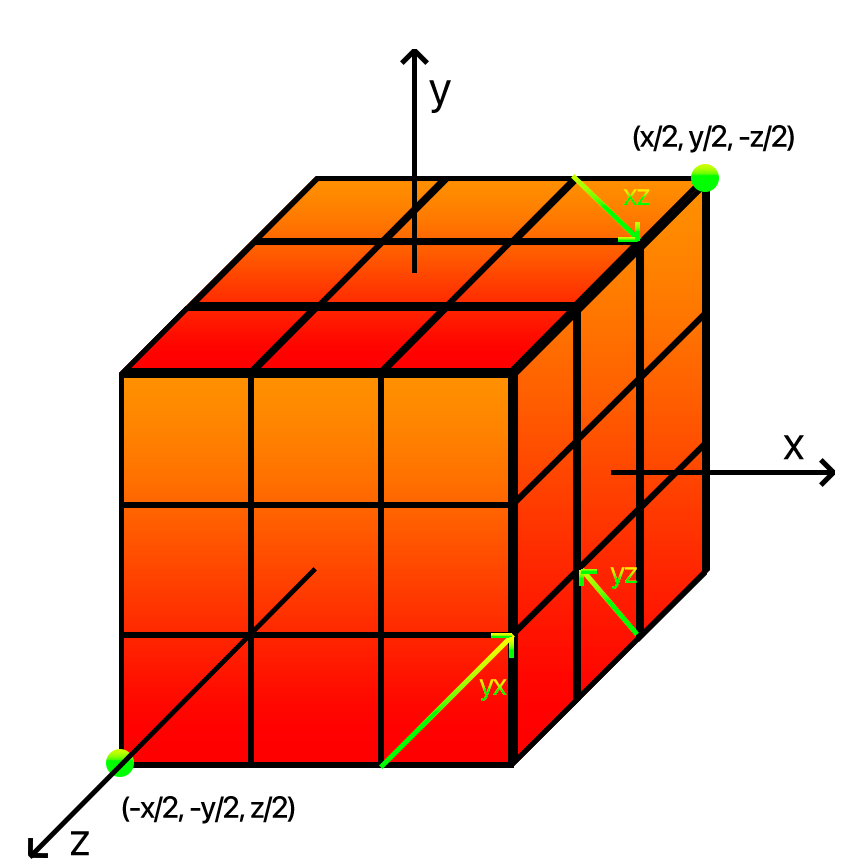
\includegraphics[width=0.5\textwidth]{images/cubo_vectors.png}  
    \caption{Vetores e pontos na caixa}
    \label{fig:box_vectors}
\end{figure}
Para facilitar as contas, o gerador converte as divisões que recebe no número de
slices que o cubo tem (\textit{slices = divisions + 1}).\\
Em seguida são definidos 3 vetores cada um associado a um dos planos que
atravessam os eixos e têm como coordenadas o comprimento de cada uma das slices
do cubo.\\
\begin{lstlisting}
float stepx = _x / _slices;
float stepy = _y / _slices;
float stepz = _z / _slices;

Vector xy = Vector(stepx, stepy,     0);
Vector yz = Vector(0    , stepy, stepz);
Vector xz = Vector(stepx,     0, stepz);
\end{lstlisting}
Para obter os pontos ao longo de cada face utilizamos o produto de
\textit{haramard} sobre os vetores definidos anteriormente. Esta operação é
definida para duas matrizes com as mesmas dimensões e produz uma matriz onde
cada elemento (i, j) é o produto de elementos (i , j) das duas matrizes
originais. isto permite escalar os vetores apenas num eixo.\\
Assim, o código para desenhar a face da frente da caixa fica da seguinte forma,
sendo que o código para as restantes faces segue a mesma lógica:
\begin{lstlisting}
for(i32 i = 0; i < _slices; i++) {
    for(i32 j = 0; j < _slices; j++) {
        //front
        coords.push_back(front + xy.hadamard(i  , j  , 0));
        coords.push_back(front + xy.hadamard(i+1, j  , 0));
        coords.push_back(front + xy.hadamard(i+1, j+1, 0));
        coords.push_back(front + xy.hadamard(i  , j  , 0));
        coords.push_back(front + xy.hadamard(i+1, j+1, 0));
        coords.push_back(front + xy.hadamard(i  , j+1, 0));
    }
}
\end{lstlisting}

\begin{figure}[H]
    \centering 
    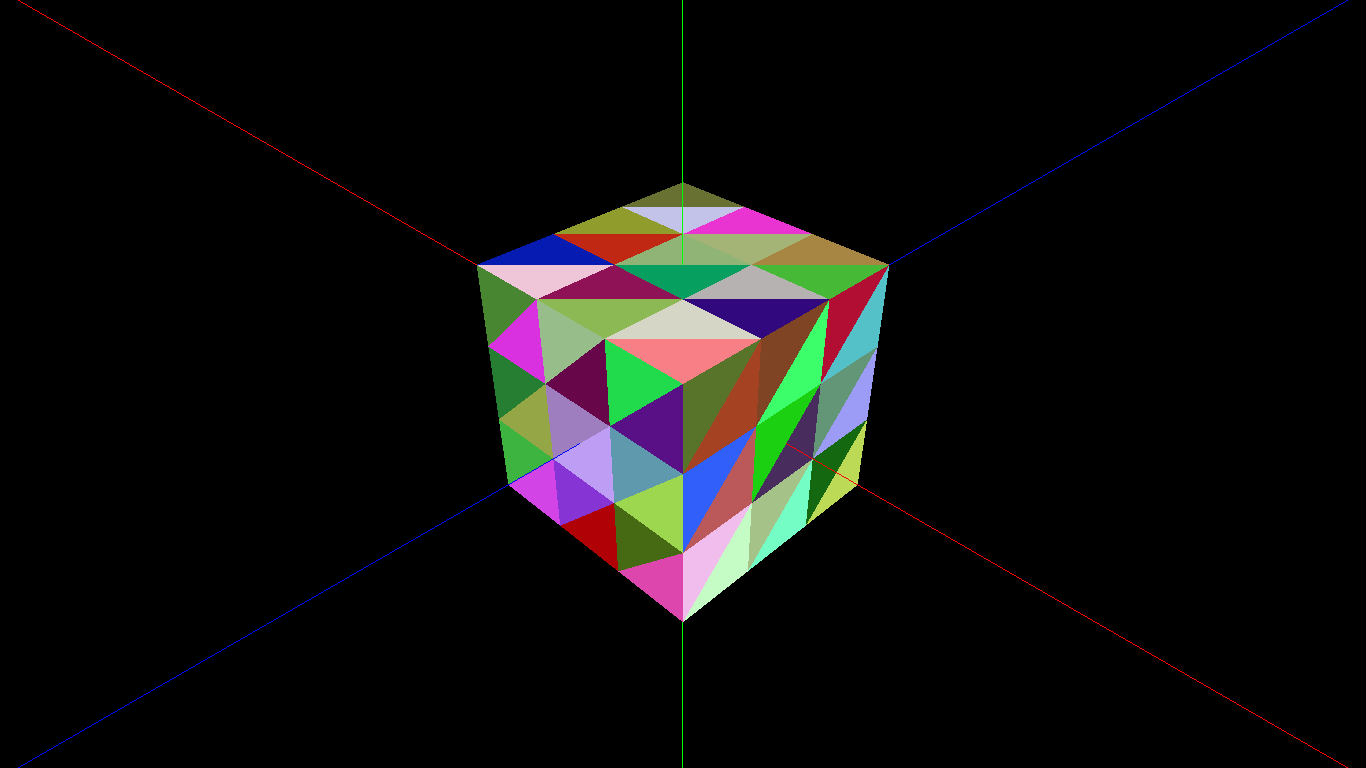
\includegraphics[width=0.5\textwidth]{images/box.png}  
    \caption{Caixa: X:5 Y:5 Z:5 Divisions:2}
    \label{fig:box_render}
\end{figure}

\section{Esfera}
Para desenhar a esfera é necessário saber o seu raio (\textit{\_radius}), o
número de slices (\textit{\_slices}) e o número de stacks (\textit{\_stacks}).\\
Fizemos uso do sistema de coordenadas esféricas definidas
anteriormente para desenhar a esfera. Como o próprio nome indica, o espaço
definido por estas coordenadas é esférico o que facilita o desenho de uma
esfera.\\
Tal como foi referido, um ponto precisa de três valores para ser defenido num
sistema de coordenadas esféricas. O primeiro é a distância ao ponto do centro do
referencial que por definição também é o raio da esfera. Assim basta obter a
inclinação e o azimute.\\
Para facilitar estas contas são calculados dois valores:\\
O angulo entre cada slice (ang\_slice = 2 * $\pi$ / n de slices) e o angulo
entre cada stack (ang\_stack = $\pi$ / n de stacks).\\
\begin{figure}[H]
    \centering 
    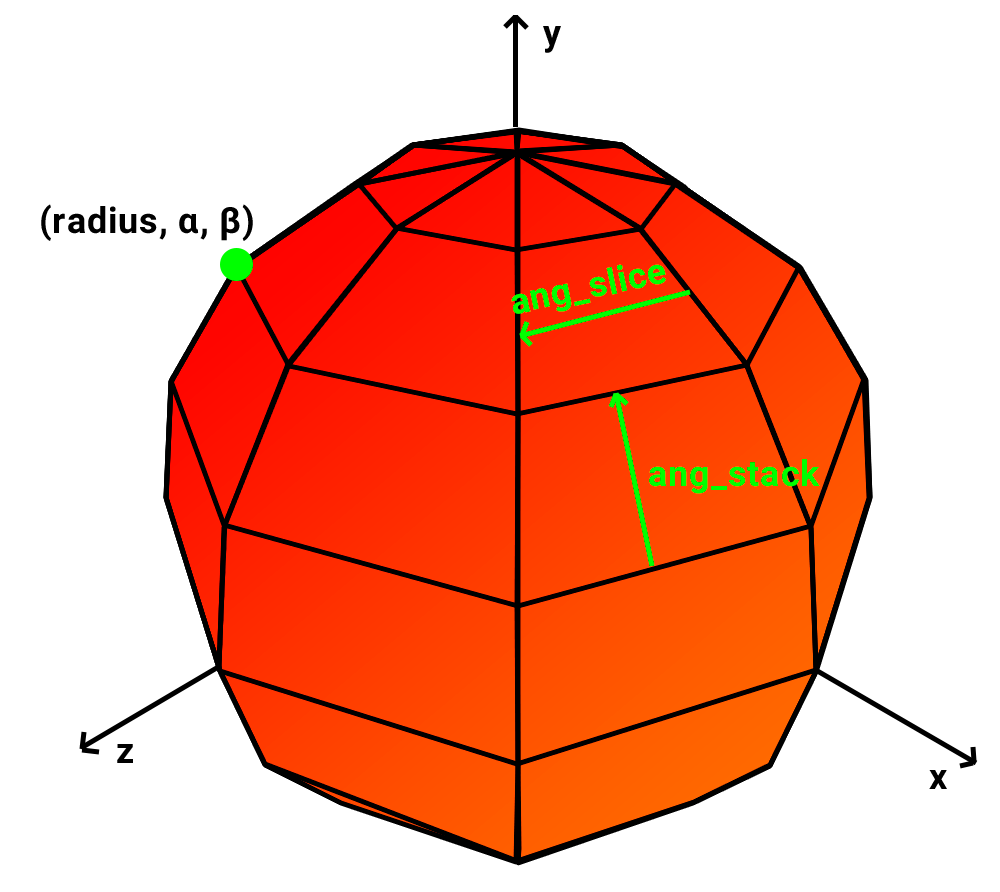
\includegraphics[width=0.5\textwidth]{images/sphere_vetores.png}  
    \caption{Angulos e pontos na esfera}
    \label{fig:sphere}
\end{figure}
Assim, para obter todos os pontos numa esfera podemos usar o excerto de código:

\begin{lstlisting}
for(i32 slice = 0; slice < _slices; slice++)
    for(i32 stack = 0; stack < _stacks; stack++)
        coords.push_back(
            PointSpherical(_radius, ang_stack * stack, ang_slice * slice));
\end{lstlisting}

Para obter os próximos pontos da esfera de forma a criar os triângulos basta
fazer \textit{ang\_stack * (stack + 1)} e \textit{ang\_slice * (slice + 1)}\\
Assim, juntando estes quatro pontos com o explicado na criação do plano:

\begin{lstlisting}
for(i32 slice = 0; slice < _slices; slice++)
    for(i32 stack = 0; stack < _stacks; stack++) {
        //1st triangle
        coords.push_back(
            PointSpherical(_radius, ang_stack * (stack+1), ang_slice * (slice+1)));
        coords.push_back(
            PointSpherical(_radius, ang_stack * stack, ang_slice * (slice+1)));
        coords.push_back(
            PointSpherical(_radius, ang_stack * stack, ang_slice * slice));
        //2nd triangle
        coords.push_back(
            PointSpherical(_radius, ang_stack * (stack+1), ang_slice * slice));
        coords.push_back(
            PointSpherical(_radius, ang_stack * (stack+1), ang_slice
        * (slice+1)));
        coords.push_back(
            PointSpherical(_radius, ang_stack * stack, ang_slice
        * slice));
        }
\end{lstlisting}

O resultado deste código já gera uma esfera. No entanto, quando es está a
desenhar a primeira e a última stack os triângulos são duplicados.
Para resolver este problema basta não desenhar um dos triângulos nestes casos.
Assim a versão final fica:

\begin{lstlisting}
for(i32 slice = 0; slice < _slices; slice++)
    for(i32 stack = 0; stack < _stacks; stack++) {
        if(! (stack == 0 || stack == stacks-1)) {
            //1st triangle
            coords.push_back(
                PointSpherical(_radius, ang_stack * (stack+1), ang_slice * (slice+1)));
            coords.push_back(
                PointSpherical(_radius, ang_stack * stack, ang_slice * (slice+1)));
            coords.push_back(
                PointSpherical(_radius, ang_stack * stack, ang_slice * slice));
        }
        //2nd triangle
        coords.push_back(
            PointSpherical(_radius, ang_stack * (stack+1), ang_slice * slice));
        coords.push_back(
            PointSpherical(_radius, ang_stack * (stack+1), ang_slice * (slice+1)));
        coords.push_back(
            PointSpherical(_radius, ang_stack * stack, ang_slice * slice));
    }
\end{lstlisting}


\begin{figure}[H]
    \centering 
    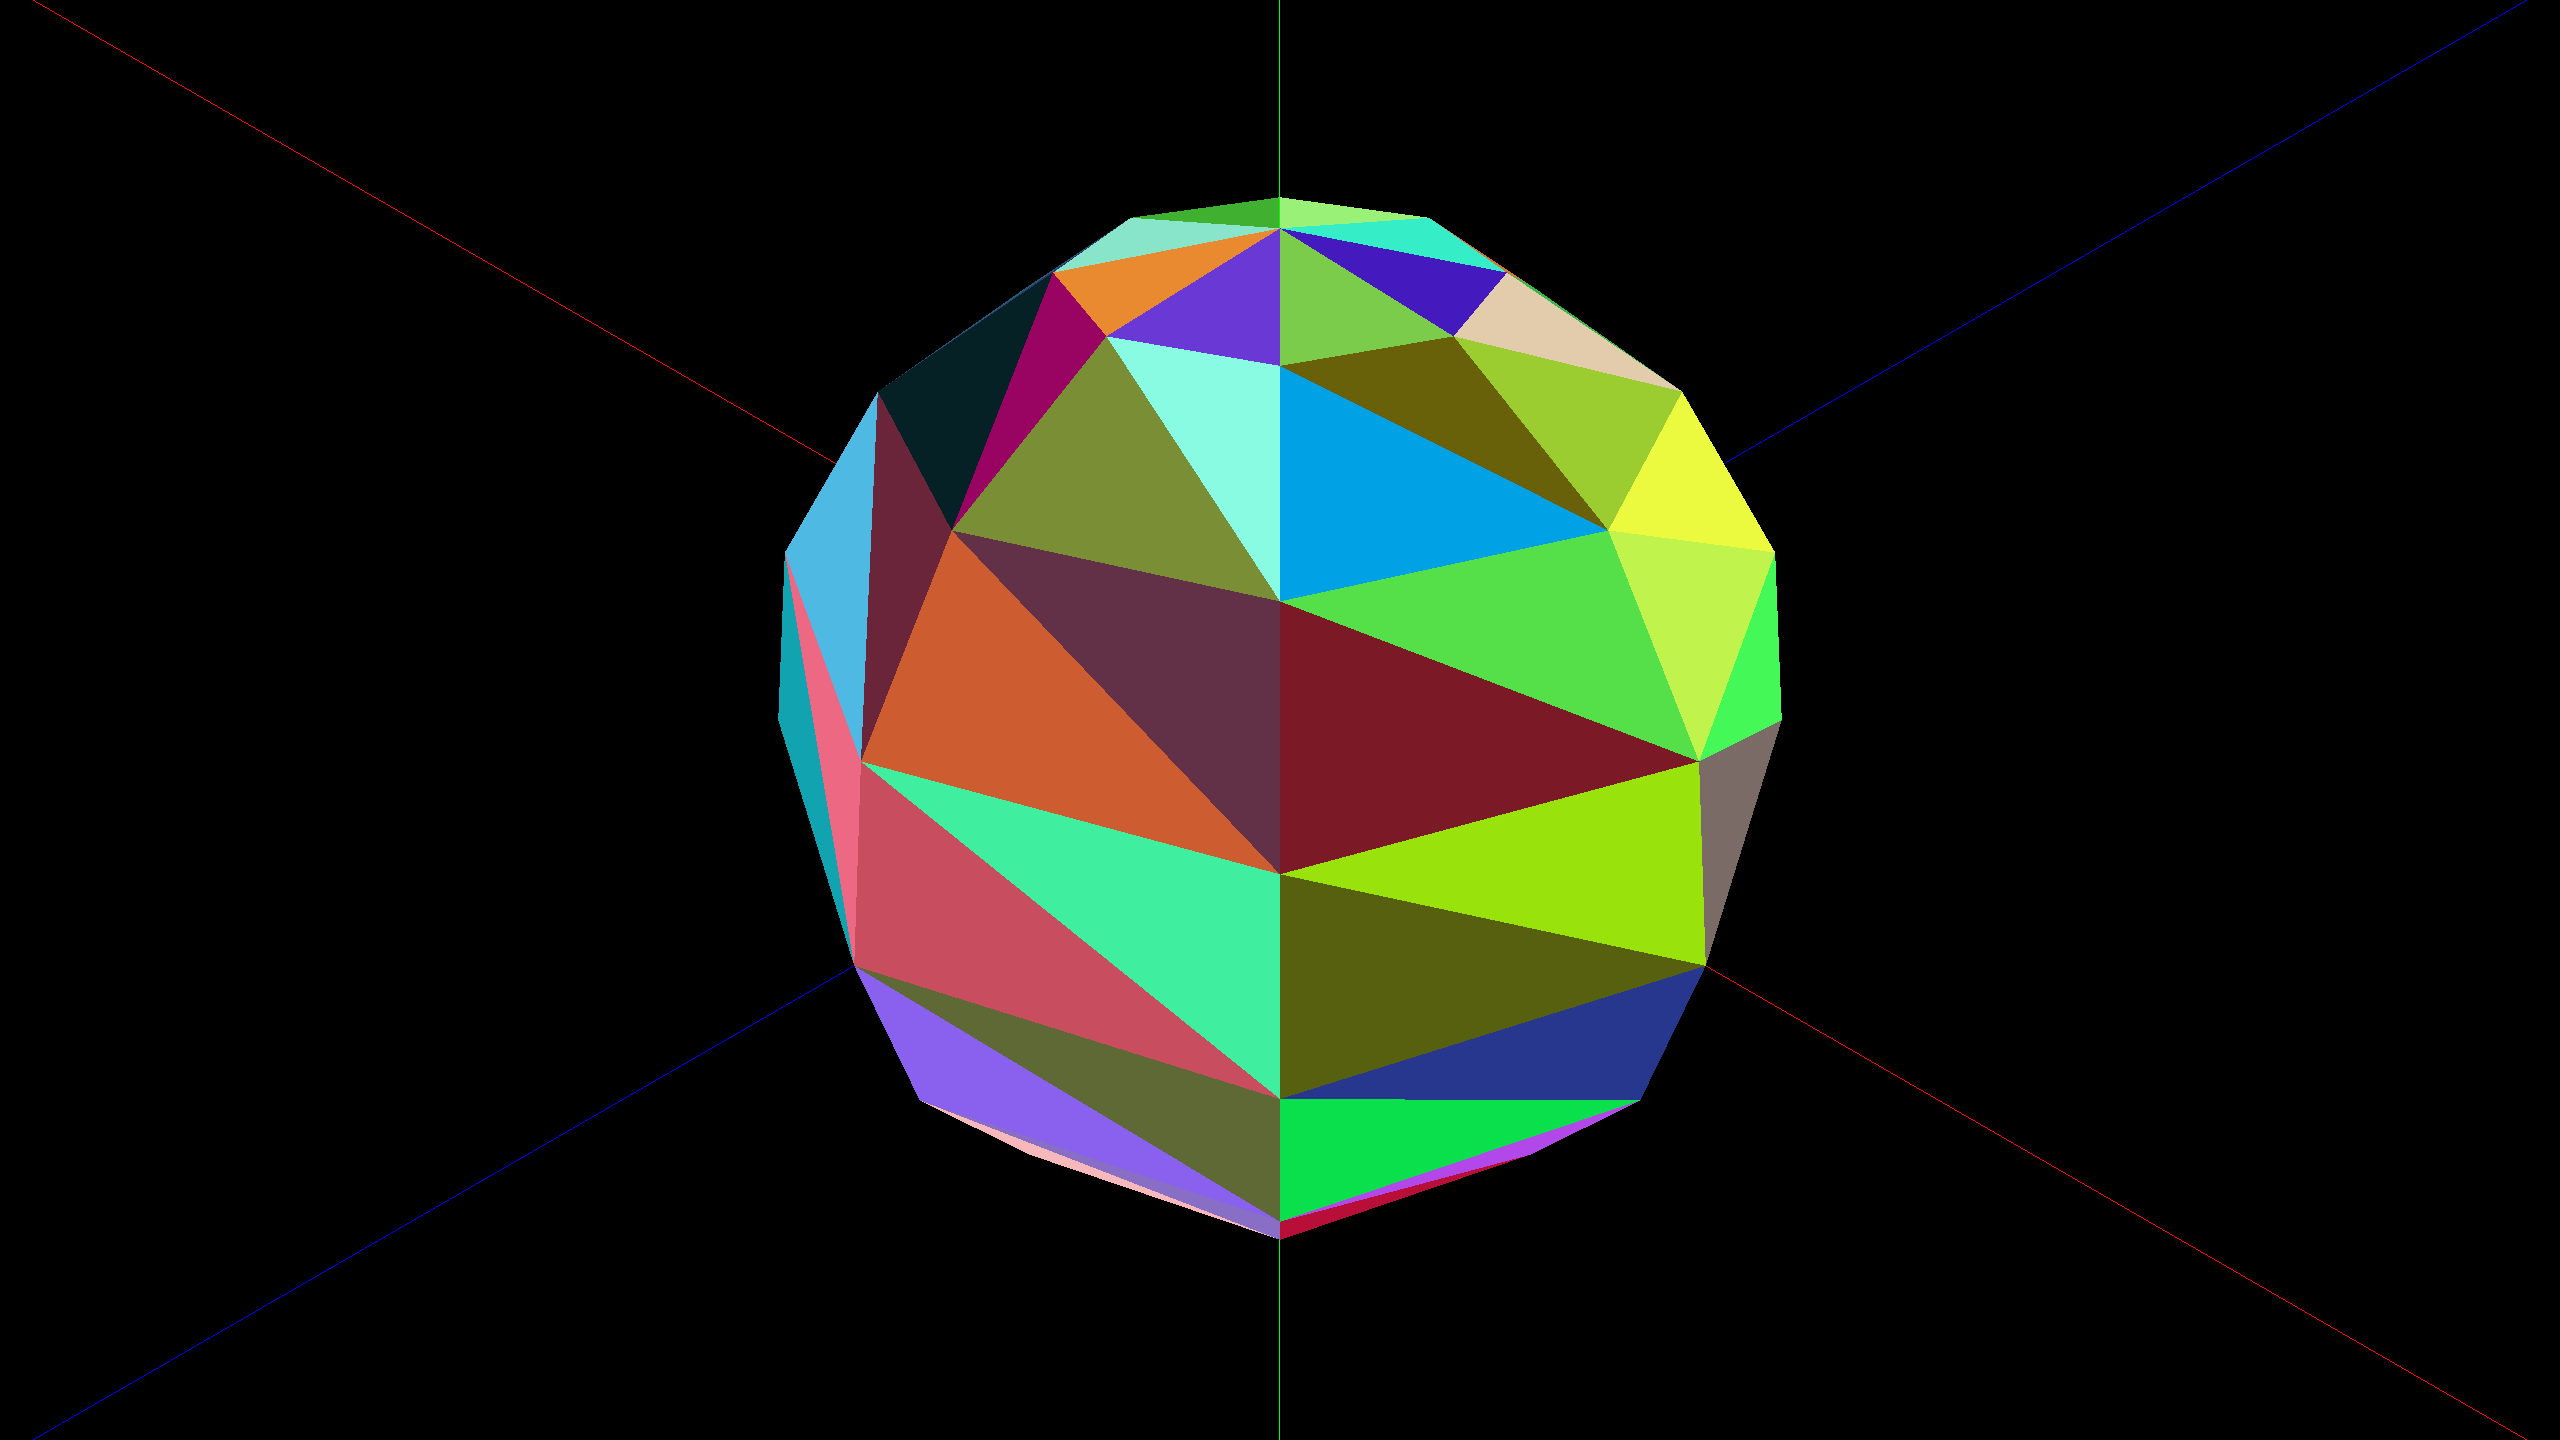
\includegraphics[width=0.5\textwidth]{images/sphere.png}  
    \caption{Esfera: raio:5 slices:8 stacks:8}
    \label{fig:cilindro_render}
\end{figure}


\section{Cone}
Para desenhar um cone é necessário saber o seu raio (\textit{\_radius}), a sua
altura (\textit{\_height}), o número de slices (\textit{\_slices}) e o número de
stacks (\textit{\_stacks}).\\
Primeiramente é calculado o ângulo entre cada slice (\textit(ang\_slice))
e é definido um ponto que se encontra no topo do cone (\textit{top\_point}).

\begin{lstlisting}
float ang_slice = 2 * M_PI / _slices;
Point top_point = Point(0, _height, 0);
\end{lstlisting}
\begin{figure}[H]
    \centering 
    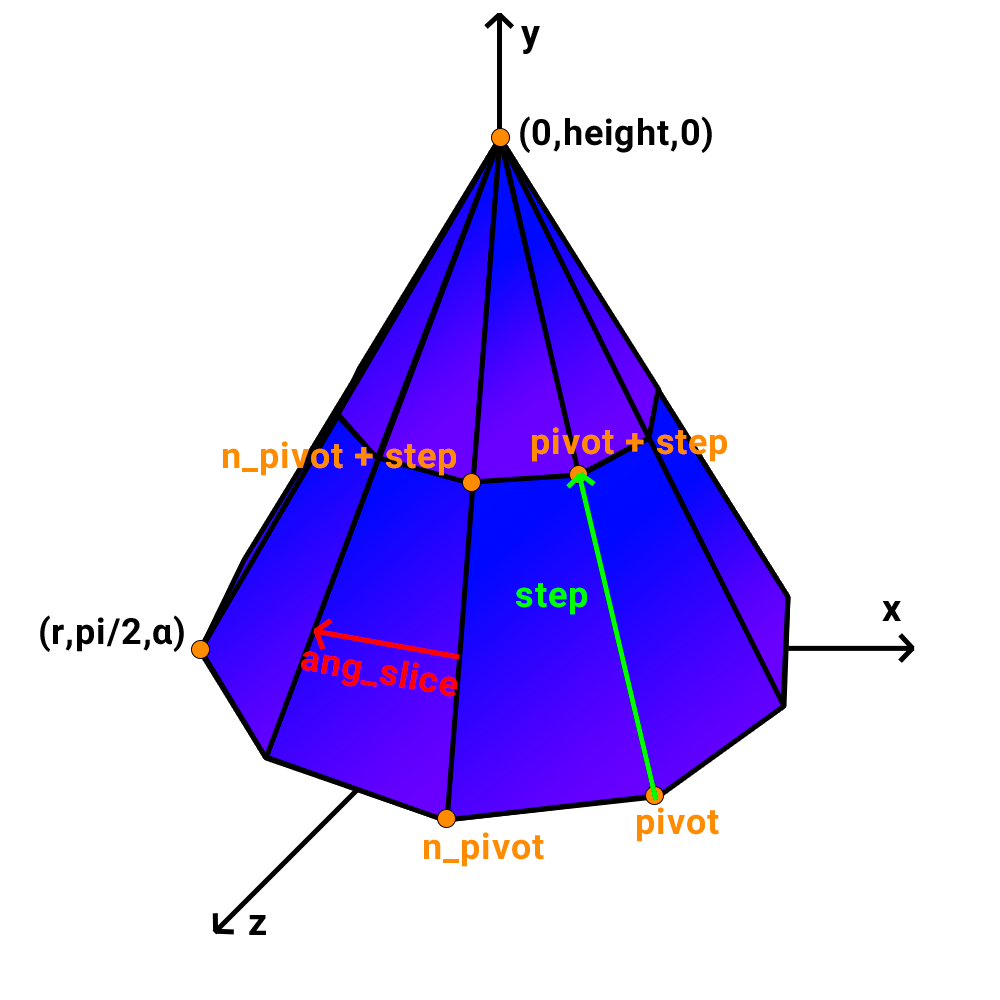
\includegraphics[width=0.5\textwidth]{images/cone_vetores.png}  
    \caption{pontos e vetores no cone}
    \label{fig:cone_vetores}
\end{figure}
Assim, os pontos na base do cone são da forma \textit{(radius, $\pi$, a)}.
Logo para desenhar a base do cone fazemos:

\begin{lstlisting}
for(i32 slice = 0; slice < _slices; slice++) {
    Point base   = PointSpherical(_radius, M_PI/2, ang_slice *  slice);
    Point n_base = PointSpherical(_radius, M_PI/2, ang_slice * (slice+1));

    coords.push_back(n_base);
    coords.push_back(base);
    coords.push_back(PointSpherical(0, 0, 0));

}
\end{lstlisting}
Em seguida é calculado em cada ciclo um vetor que vai do \textit{base} e do
\textit{n\_base} até ao topo do cone mas que só tem o comprimento de uma stack:

\begin{lstlisting}
Vector step   = Vector(  base, top_point) / _stacks;
Vector n_step = Vector(n_base, top_point) / _stacks;
\end{lstlisting}
Assim, para obter um ponto na lateral do cone podemos fazer \textit{base + step
* stack}. Visto que no topo do cone os triângulos também se iriam sobrepor uma
solução semelhante à usada na esfera foi aplicada.\\
Assim, o código final fica:

\begin{lstlisting}
for(i32 slice = 0; slice < _slices; slice++) {
    Point base   = PointSpherical(_radius, M_PI/2, ang_slice *  slice);
    Point n_base = PointSpherical(_radius, M_PI/2, ang_slice * (slice+1));

    coords.push_back(n_base);
    coords.push_back(base);
    coords.push_back(Point(0, 0, 0));

    Vector step   = Vector(  base, top_point) / _stacks;
    Vector n_step = Vector(n_base, top_point) / _stacks;

    for(i32 stack = 0; stack < _stacks; stack++) {
        Point pivot   =    base +   step * stack;
        Point n_pivot =  n_base + n_step * stack;

        if(!(stack == _stacks -1)) {
            coords.push_back(pivot);
            coords.push_back(n_pivot + n_step);
            coords.push_back(pivot + step);
        }
        coords.push_back(pivot);
        coords.push_back(n_pivot);
        coords.push_back(n_pivot + n_step);
    }
}
\end{lstlisting}

\begin{figure}[H]
    \centering 
    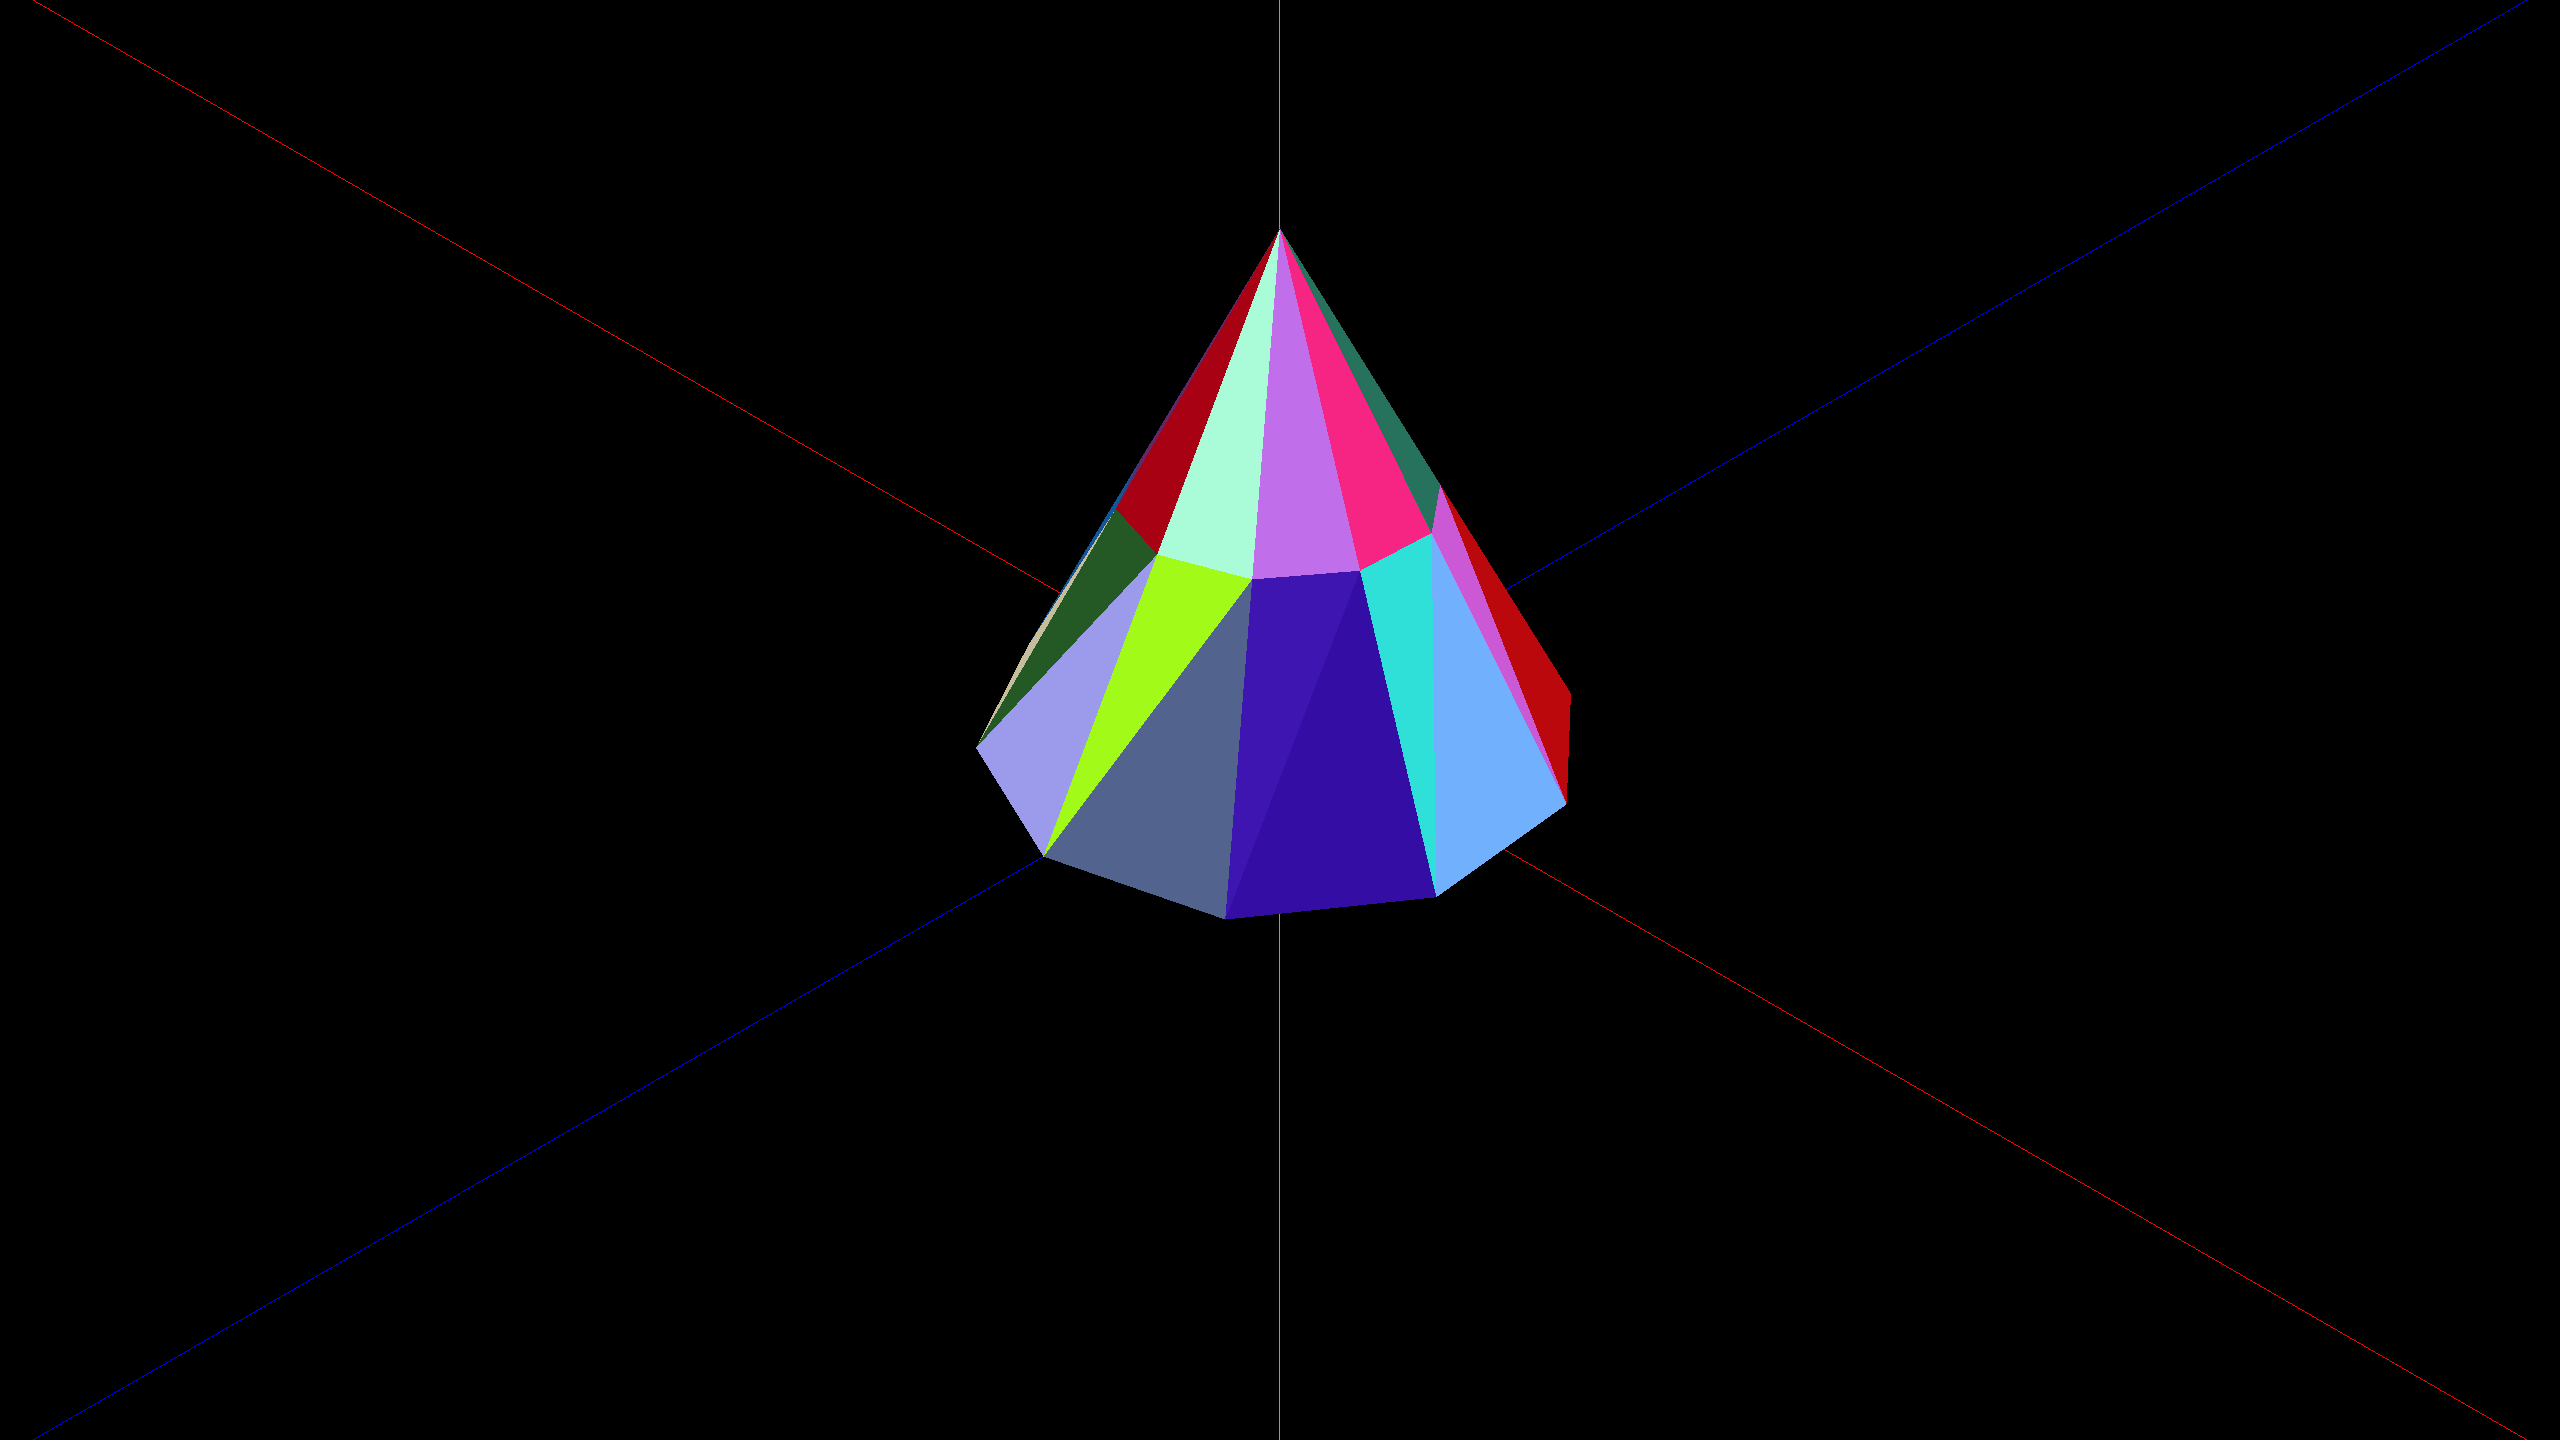
\includegraphics[width=0.5\textwidth]{images/cone.png}  
    \caption{Cilindro: altura:5 raio:3 slices:10 stacks:2}
    \label{fig:cilindro_render}
\end{figure}

\section{Cilindro}
Para desenhar o cilindro primeiro é definido um vetor que vai da base do cone ao
topo do cone(top) e um vetor que tem a altura de uma stack do cilindro(step) e
é calculado o ângulo que uma slice tem(ang\_slice).\\
Assim, para um ponto da aresta da base é dado por \textit{(radius, $\pi$/2,
ang\_slice * slice)}.
\begin{lstlisting}
Vector top = Vector(0, _height, 0);
Vector step = top / _stacks;
float ang_slice = 2 * M_PI / _slices;
\end{lstlisting}
\begin{figure}[H]
    \centering 
    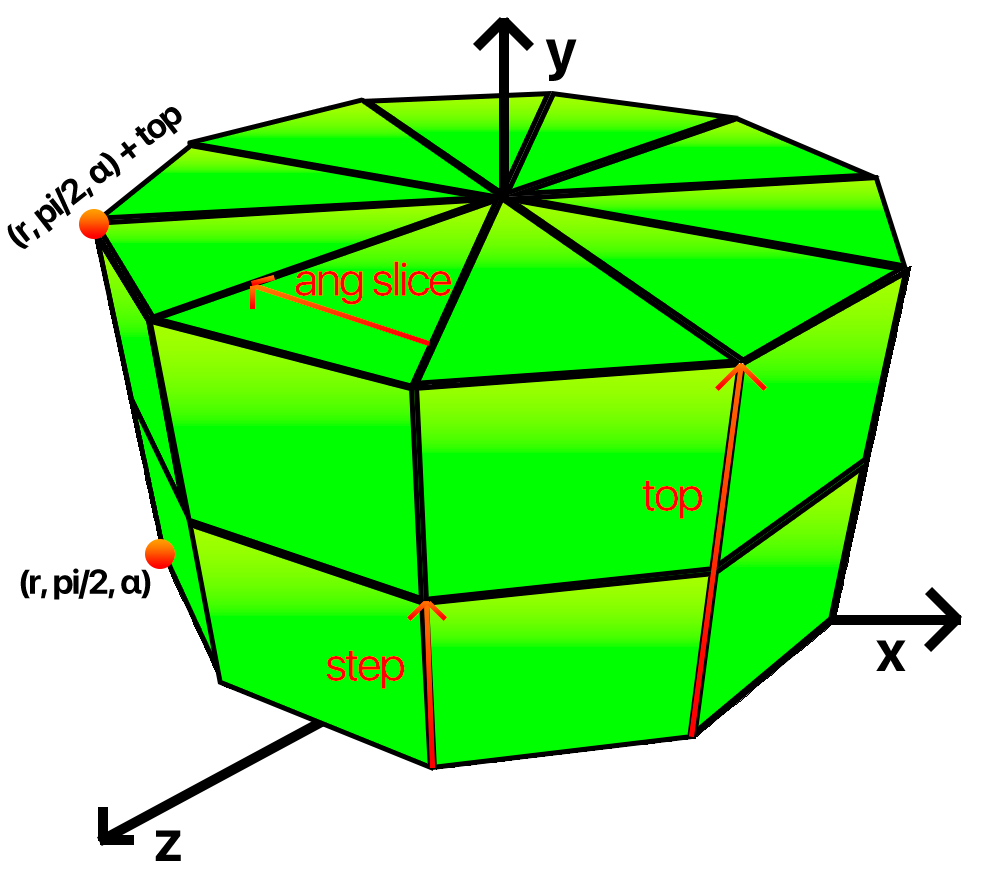
\includegraphics[width=0.5\textwidth]{images/cilindro_vetores.png}  
    \caption{Vetores e ângulos dos cilindros}
    \label{fig:cilindro_vec}
\end{figure}
Assim para desenhar a base do cilindro e o topo do cilindro fazemos:

\begin{lstlisting}
for(i32 slice = 0; slice < _slices; slice++) {
    PointSpherical central = PointSpherical(0, 0, 0);
    PointSpherical base    = PointSpherical(_radius, M_PI/2, ang_slice * slice);
    PointSpherical n_base  = PointSpherical(_radius, M_PI/2, ang_slice *(slice+1));
    //top & bottom
    coords.push_back(n_base);
    coords.push_back(base);
    coords.push_back(central);
    coords.push_back(central + top);
    coords.push_back(base + top);
    coords.push_back(n_base + top);
}
\end{lstlisting}

Para desenhar as laterais do cilindro coloca-se um ciclo for dentro do
ciclo definido anteriormente de forma a percorrer as stacks do sólido.
Assim, a versão final do código fica:

\begin{lstlisting}
for(i32 slice = 0; slice < _slices; slice++) {
    PointSpherical central = PointSpherical(0, 0, 0);
    PointSpherical base    = PointSpherical(_radius, M_PI/2, ang_slice * slice);
    PointSpherical n_base  = PointSpherical(_radius, M_PI/2, ang_slice *(slice+1));
    //top & bottom
    coords.push_back(n_base);
    coords.push_back(base);
    coords.push_back(central);
    coords.push_back(central + top);
    coords.push_back(base + top);
    coords.push_back(n_base + top);

    //side
    for(i32 stack = 0; stack < _stacks; stack++) {
        Point pivot   =   base + step * stack;
        Point n_pivot = n_base + step * stack;

        coords.push_back(pivot);
        coords.push_back(n_pivot + step);
        coords.push_back(pivot + step);
        coords.push_back(pivot);
        coords.push_back(n_pivot);
        coords.push_back(n_pivot + step);
    }
}
\end{lstlisting}



\begin{figure}[H]
    \centering 
    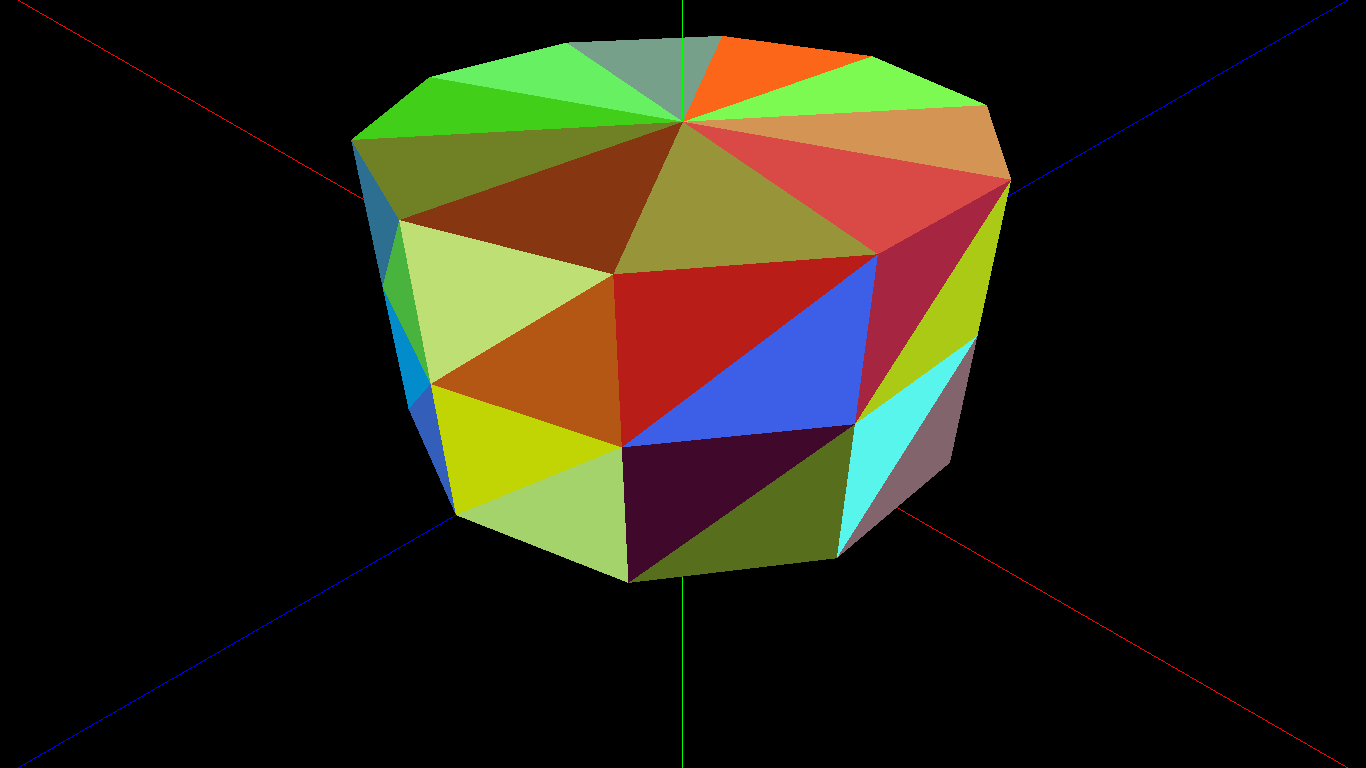
\includegraphics[width=0.5\textwidth]{images/cylinder.png}  
    \caption{Cilindro: altura:5 raio:5 slices:10 stacks:2}
    \label{fig:cilindro_render}
\end{figure}

\chapter{Engine}
Neste módulo foi desenvolvido um motor 3D simples.\\
Quando se executa o progrma gerado por defeito é aberta a scene guardada em
\textit{scenes/config.xml}. Se alguém ficehiro for passado como argumento esse
será o selecionado.\\
Como ainda não existem sombras e luz as formas não são facilmente
distinguíveis. De forma a resolver este problema decidimos atribuir a cada
triângulo uma cor aleatória.
\begin{figure}[H]
    \centering 
    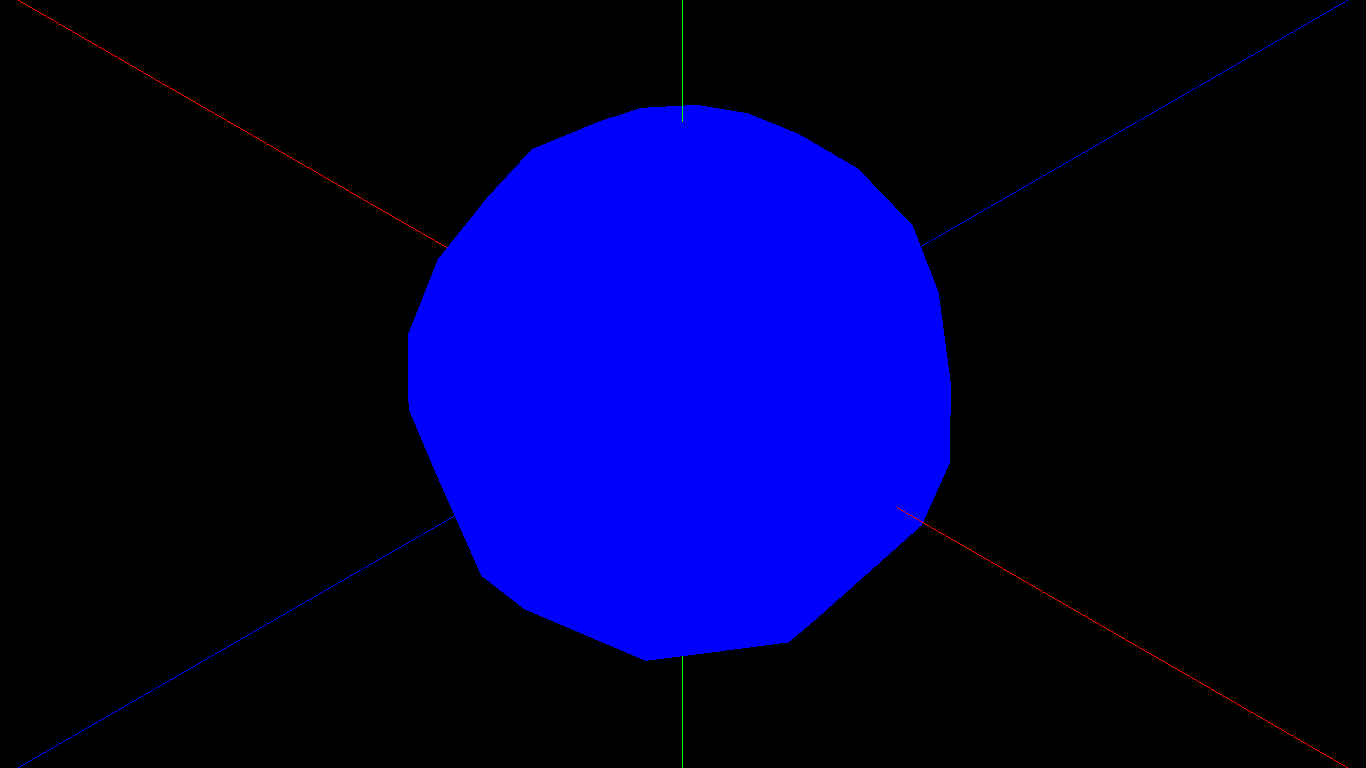
\includegraphics[width=0.5\textwidth]{images/sphere_onecolor.png}  
    \caption{Esfera com cor sólida}
    \label{fig:sphere_color}
\end{figure}
\begin{figure}[H]
    \centering 
    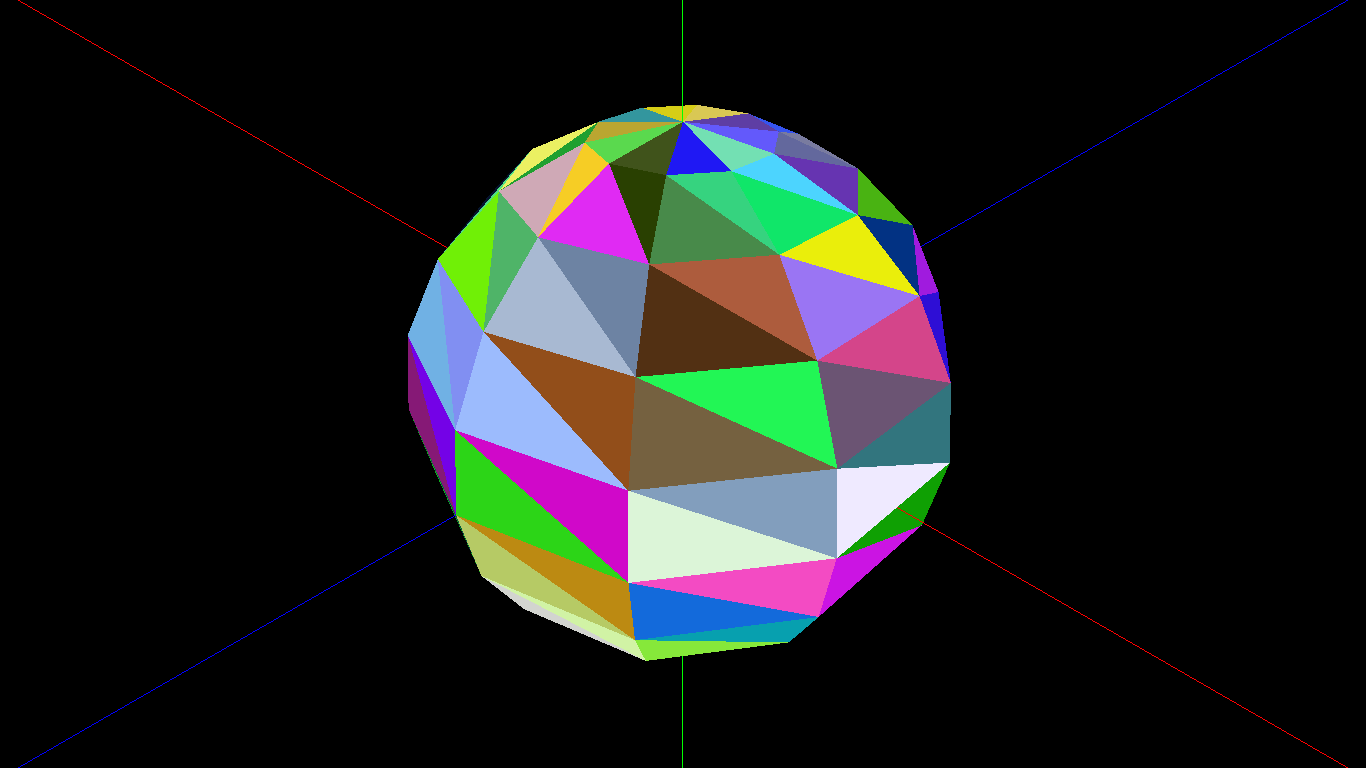
\includegraphics[width=0.5\textwidth]{images/sphere_color.png}  
    \caption{Esfera com várias cores por triângulo}
    \label{fig:sphere_onecolor}
\end{figure}

\section{3D Model loading}
Para facilitar a leitura do ficheiro final gerado pelo gerador foi desenvolvida
uma classe denominada de \textit{Model}. Esta contem um vetor de pontos que são
carregados do ficheiro anteriormente gerado e para o povoar apenas é necessário
indicar o nome do ficheiro.\\
\begin{lstlisting}
Model::Model(string fileName){
    float x, y, z;
    ifstream file(fileName.c_str());
    while (file >> x >> y >> z)
         points.push_back(Point(x, y, z));
}
\end{lstlisting}
Esta classe também contém um método para desenhar o modelo \textit{draw\_model} que chama um método
para desenhar triângulos com cores aleatórias \textit{draw\_triangle}.
\begin{lstlisting}
void draw_triangle(Point p1, Point p2, Point p3){
    float r = static_cast <float> (rand()) / static_cast <float> (RAND_MAX);
    float g = static_cast <float> (rand()) / static_cast <float> (RAND_MAX);
    float b = static_cast <float> (rand()) / static_cast <float> (RAND_MAX);
    glColor3f(r, g, b);
    glBegin(GL_TRIANGLES);
        glVertex3f(p1.x(), p1.y(), p1.z());
        glVertex3f(p2.x(), p2.y(), p2.z());
        glVertex3f(p3.x(), p3.y(), p3.z());
    glEnd();
}

void Model::draw_model() {
    for(i32 i = 0; i < points.size(); i += 3)
        draw_triangle(points[i], points[i+1], points[i+2]);
}
\end{lstlisting}

\section{XML parsing}
Para dar parsing ao XML utilizamos a biblioteca \textit{rapidxml}. Nesta
primeira versão do parser apenas obtemos quais são os ficheiros dos modelos a
carregar contidos no xml. De forma a garantir que o ficheiro é lido apenas uma
vez o carregamento é feito imediatamente quando o programa inicia e os ficheiros
são carregas para a classe \textit{Models} que contem um vetor de \textit{Model}
e o resultado é guardado num singleton.\\
Assim, para carregar todos os sólidos dentro do xml basta fazer:
\begin{lstlisting}
models = Models(read_models(sceneName));
\end{lstlisting}
Para desenhar os modelos utilizamos o método \textit{draw\_models()}.

\section{Camera}
A camera consiste em dois pontos. Um ponto de coordenadas esféricas que
representa a localização da camera no espaço e um ponto de coordenadas
cartesianas que representa para onde a camera está a olhar.\\
\begin{lstlisting}
PointSpherical _pl;
Point _center;
\end{lstlisting}
Para desenhar a camera converte se o ponto esférico num ponto cartesiano e
utiliza-se a função \textit{gluLookAt}.
\begin{lstlisting}
Point c = Point(_pl);
glLoadIdentity();
gluLookAt(c.x(),c.y(),c.z(), 
	_center.x(),_center.y(),_center.z(),
		0.0f,1.0f,0.0f);
\end{lstlisting}
Para mover a camera basta utilizar as funções definidas na classe \textit{Point}
e \textit{PointSpherical} para alterar a posição da camera.

\chapter{Conclusão}
Com este trabalho prático podemos aplicar os conhecimentos lecionados até agora
nas aulas da unidade curricular de computação gráfica permitindo assim que
aprofundar os nossos conhecimentos de openGl.\\
Como trabalho futuro gostaríamos de melhorar a camera de orbita que foi
implementada no \textit{engine}, introduzir mais cameras distintas e criar mais
primitivas no \textit{generator} como a torus, por exemplo.

\end{document}
